
%% bare_conf_compsoc.tex
%% V1.4b
%% 2015/08/26
%% by Michael Shell
%% See:
%% http://www.michaelshell.org/
%% for current contact information.
%%
%% This is a skeleton file demonstrating the use of IEEEtran.cls
%% (requires IEEEtran.cls version 1.8b or later) with an IEEE Computer
%% Society conference paper.
%%
%% Support sites:
%% http://www.michaelshell.org/tex/ieeetran/
%% http://www.ctan.org/pkg/ieeetran
%% and
%% http://www.ieee.org/

%%*************************************************************************
%% Legal Notice:
%% This code is offered as-is without any warranty either expressed or
%% implied; without even the implied warranty of MERCHANTABILITY or
%% FITNESS FOR A PARTICULAR PURPOSE! 
%% User assumes all risk.
%% In no event shall the IEEE or any contributor to this code be liable for
%% any damages or losses, including, but not limited to, incidental,
%% consequential, or any other damages, resulting from the use or misuse
%% of any information contained here.
%%
%% All comments are the opinions of their respective authors and are not
%% necessarily endorsed by the IEEE.
%%
%% This work is distributed under the LaTeX Project Public License (LPPL)
%% ( http://www.latex-project.org/ ) version 1.3, and may be freely used,
%% distributed and modified. A copy of the LPPL, version 1.3, is included
%% in the base LaTeX documentation of all distributions of LaTeX released
%% 2003/12/01 or later.
%% Retain all contribution notices and credits.
%% ** Modified files should be clearly indicated as such, including  **
%% ** renaming them and changing author support contact information. **
%%*************************************************************************


% *** Authors should verify (and, if needed, correct) their LaTeX system  ***
% *** with the testflow diagnostic prior to trusting their LaTeX platform ***
% *** with production work. The IEEE's font choices and paper sizes can   ***
% *** trigger bugs that do not appear when using other class files.       ***                          ***
% The testflow support page is at:
% http://www.michaelshell.org/tex/testflow/


\documentclass[11pt,journal,compsoc]{IEEEtran}
% Some/most Computer Society conferences require the compsoc mode option,
% but others may want the standard conference format.
%
% If IEEEtran.cls has not been installed into the LaTeX system files,
% manually specify the path to it like:
% \documentclass[conference,compsoc]{../sty/IEEEtran}





% Some very useful LaTeX packages include:
% (uncomment the ones you want to load)


% *** MISC UTILITY PACKAGES ***
%
%\usepackage{ifpdf}
% Heiko Oberdiek's ifpdf.sty is very useful if you need conditional
% compilation based on whether the output is pdf or dvi.
% usage:
% \ifpdf
%   % pdf code
% \else
%   % dvi code
% \fi
% The latest version of ifpdf.sty can be obtained from:
% http://www.ctan.org/pkg/ifpdf
% Also, note that IEEEtran.cls V1.7 and later provides a builtin
% \ifCLASSINFOpdf conditional that works the same way.
% When switching from latex to pdflatex and vice-versa, the compiler may
% have to be run twice to clear warning/error messages.






% *** CITATION PACKAGES ***
%
\ifCLASSOPTIONcompsoc
  % IEEE Computer Society needs nocompress option
  % requires cite.sty v4.0 or later (November 2003)
  \usepackage[nocompress]{cite}
\else
  % normal IEEE
  \usepackage{cite}
\fi
% cite.sty was written by Donald Arseneau
% V1.6 and later of IEEEtran pre-defines the format of the cite.sty package
% \cite{} output to follow that of the IEEE. Loading the cite package will
% result in citation numbers being automatically sorted and properly
% "compressed/ranged". e.g., [1], [9], [2], [7], [5], [6] without using
% cite.sty will become [1], [2], [5]--[7], [9] using cite.sty. cite.sty's
% \cite will automatically add leading space, if needed. Use cite.sty's
% noadjust option (cite.sty V3.8 and later) if you want to turn this off
% such as if a citation ever needs to be enclosed in parenthesis.
% cite.sty is already installed on most LaTeX systems. Be sure and use
% version 5.0 (2009-03-20) and later if using hyperref.sty.
% The latest version can be obtained at:
% http://www.ctan.org/pkg/cite
% The documentation is contained in the cite.sty file itself.
%
% Note that some packages require special options to format as the Computer
% Society requires. In particular, Computer Society  papers do not use
% compressed citation ranges as is done in typical IEEE papers
% (e.g., [1]-[4]). Instead, they list every citation separately in order
% (e.g., [1], [2], [3], [4]). To get the latter we need to load the cite
% package with the nocompress option which is supported by cite.sty v4.0
% and later.




% *** GRAPHICS RELATED PACKAGES ***
%
\ifCLASSINFOpdf
  % \usepackage[pdftex]{graphicx}
  % declare the path(s) where your graphic files are
  % \graphicspath{{../pdf/}{../jpeg/}}
  % and their extensions so you won'\left\lbrace t have to specify these with
  % every instance of \includegraphics
  % \DeclareGraphicsExtensions{.pdf,.jpeg,.png}
\else
  % or other class option (dvipsone, dvipdf, if not using dvips). graphicx
  % will default to the driver specified in the system graphics.cfg if no
  % driver is specified.
  % \usepackage[dvips]{graphicx}
  % declare the path(s) where your graphic files are
  % \graphicspath{{../eps/}}
  % and their extensions so you won't have to specify these with
  % every instance of \includegraphics
  % \DeclareGraphicsExtensions{.eps}
\fi
% graphicx was written by David Carlisle and Sebastian Rahtz. It is
% required if you want graphics, photos, etc. graphicx.sty is already
% installed on most LaTeX systems. The latest version and documentation
% can be obtained at: 
% http://www.ctan.org/pkg/graphicx
% Another good source of documentation is "Using Imported Graphics in
% LaTeX2e" by Keith Reckdahl which can be found at:
% http://www.ctan.org/pkg/epslatex
%
% latex, and pdflatex in dvi mode, support graphics in encapsulated
% postscript (.eps) format. pdflatex in pdf mode supports graphics
% in .pdf, .jpeg, .png and .mps (metapost) formats. Users should ensure
% that all non-photo figures use a vector format (.eps, .pdf, .mps) and
% not a bitmapped formats (.jpeg, .png). The IEEE frowns on bitmapped formats
% which can result in "jaggedy"/blurry rendering of lines and letters as
% well as large increases in file sizes.
%
% You can find documentation about the pdfTeX application at:
% http://www.tug.org/applications/pdftex





% *** MATH PACKAGES ***
%
%\usepackage{amsmath}
% A popular package from the American Mathematical Society that provides
% many useful and powerful commands for dealing with mathematics.
%
% Note that the amsmath package sets \interdisplaylinepenalty to 10000
% thus preventing page breaks from occurring within multiline equations. Use:
%\interdisplaylinepenalty=2500
% after loading amsmath to restore such page breaks as IEEEtran.cls normally
% does. amsmath.sty is already installed on most LaTeX systems. The latest
% version and documentation can be obtained at:
% http://www.ctan.org/pkg/amsmath





% *** SPECIALIZED LIST PACKAGES ***
%
%\usepackage{algorithmic}
% algorithmic.sty was written by Peter Williams and Rogerio Brito.
% This package provides an algorithmic environment fo describing algorithms.
% You can use the algorithmic environment in-text or within a figure
% environment to provide for a floating algorithm. Do NOT use the algorithm
% floating environment provided by algorithm.sty (by the same authors) or
% algorithm2e.sty (by Christophe Fiorio) as the IEEE does not use dedicated
% algorithm float types and packages that provide these will not provide
% correct IEEE style captions. The latest version and documentation of
% algorithmic.sty can be obtained at:
% http://www.ctan.org/pkg/algorithms
% Also of interest may be the (relatively newer and more customizable)
% algorithmicx.sty package by Szasz Janos:
% http://www.ctan.org/pkg/algorithmicx




% *** ALIGNMENT PACKAGES ***
%
%\usepackage{array}
% Frank Mittelbach's and David Carlisle's array.sty patches and improves
% the standard LaTeX2e array and tabular environments to provide better
% appearance and additional user controls. As the default LaTeX2e table
% generation code is lacking to the point of almost being broken with
% respect to the quality of the end results, all users are strongly
% advised to use an enhanced (at the very least that provided by array.sty)
% set of table tools. array.sty is already installed on most systems. The
% latest version and documentation can be obtained at:
% http://www.ctan.org/pkg/array


% IEEEtran contains the IEEEeqnarray family of commands that can be used to
% generate multiline equations as well as matrices, tables, etc., of high
% quality.




% *** SUBFIGURE PACKAGES ***
%\ifCLASSOPTIONcompsoc
%  \usepackage[caption=false,font=footnotesize,labelfont=sf,textfont=sf]{subfig}
%\else
%  \usepackage[caption=false,font=footnotesize]{subfig}
%\fi
% subfig.sty, written by Steven Douglas Cochran, is the modern replacement
% for subfigure.sty, the latter of which is no longer maintained and is
% incompatible with some LaTeX packages including fixltx2e. However,
% subfig.sty requires and automatically loads Axel Sommerfeldt's caption.sty
% which will override IEEEtran.cls' handling of captions and this will result
% in non-IEEE style figure/table captions. To prevent this problem, be sure
% and invoke subfig.sty's "caption=false" package option (available since
% subfig.sty version 1.3, 2005/06/28) as this is will preserve IEEEtran.cls
% handling of captions.
% Note that the Computer Society format requires a sans serif font rather
% than the serif font used in traditional IEEE formatting and thus the need
% to invoke different subfig.sty package options depending on whether
% compsoc mode has been enabled.
%
% The latest version and documentation of subfig.sty can be obtained at:
% http://www.ctan.org/pkg/subfig




% *** FLOAT PACKAGES ***
%
%\usepackage{fixltx2e}
% fixltx2e, the successor to the earlier fix2col.sty, was written by
% Frank Mittelbach and David Carlisle. This package corrects a few problems
% in the LaTeX2e kernel, the most notable of which is that in current
% LaTeX2e releases, the ordering of single and double column floats is not
% guaranteed to be preserved. Thus, an unpatched LaTeX2e can allow a
% single column figure to be placed prior to an earlier double column
% figure.
% Be aware that LaTeX2e kernels dated 2015 and later have fixltx2e.sty's
% corrections already built into the system in which case a warning will
% be issued if an attempt is made to load fixltx2e.sty as it is no longer
% needed.
% The latest version and documentation can be found at:
% http://www.ctan.org/pkg/fixltx2e


%\usepackage{stfloats}
% stfloats.sty was written by Sigitas Tolusis. This package gives LaTeX2e
% the ability to do double column floats at the bottom of the page as well
% as the top. (e.g., "\begin{figure*}[!b]" is not normally possible in
% LaTeX2e). It also provides a command:
%\fnbelowfloat
% to enable the placement of footnotes below bottom floats (the standard
% LaTeX2e kernel puts them above bottom floats). This is an invasive package
% which rewrites many portions of the LaTeX2e float routines. It may not work
% with other packages that modify the LaTeX2e float routines. The latest
% version and documentation can be obtained at:
% http://www.ctan.org/pkg/stfloats
% Do not use the stfloats baselinefloat ability as the IEEE does not allow
% \baselineskip to stretch. Authors submitting work to the IEEE should note
% that the IEEE rarely uses double column equations and that authors should try
% to avoid such use. Do not be tempted to use the cuted.sty or midfloat.sty
% packages (also by Sigitas Tolusis) as the IEEE does not format its papers in
% such ways.
% Do not attempt to use stfloats with fixltx2e as they are incompatible.
% Instead, use Morten Hogholm'a dblfloatfix which combines the features
% of both fixltx2e and stfloats:
%
% \usepackage{dblfloatfix}
% The latest version can be found at:
% http://www.ctan.org/pkg/dblfloatfix




% *** PDF, URL AND HYPERLINK PACKAGES ***
%
%\usepackage{url}
% url.sty was written by Donald Arseneau. It provides better support for
% handling and breaking URLs. url.sty is already installed on most LaTeX
% systems. The latest version and documentation can be obtained at:
% http://www.ctan.org/pkg/url
% Basically, \url{my_url_here}.




% *** Do not adjust lengths that control margins, column widths, etc. ***
% *** Do not use packages that alter fonts (such as pslatex).         ***
% There should be no need to do such things with IEEEtran.cls V1.6 and later.
% (Unless specifically asked to do so by the journal or conference you plan
% to submit to, of course. )


% correct bad hyphenation here
\hyphenation{op-tical net-works semi-conduc-tor}
\usepackage{graphicx}
\usepackage{adjustbox}
\usepackage{float} 
\usepackage{subcaption}
\usepackage{wrapfig}
\usepackage{amssymb}
\usepackage{amsmath}
\renewcommand\IEEEkeywordsname{Keywords}

\begin{document}
% The paper headers
\markboth{Journal of Computer Society Class Files,~Vol.~22, No.~66, DECEMBER~2019}%
{Shell \MakeLowercase{\textit{et al.}}: Bare Demo of IEEEtran.cls for  Journals}
% paper title
% Titles are generally capitalized except for words such as a, an, and, as,
% at, but, by, for, in, nor, of, on, or, the, to and up, which are usually
% not capitalized unless they are the first or last word of the title.
% Linebreaks \\ can be used within to get better formatting as desired.
% Do not put math or special symbols in the title.
\title{Design of Two-digit Decimal Number Calculator Based on Verilog\\}


% author names and affiliations
% use a multiple column layout for up to three different
% affiliations
\author{\IEEEauthorblockN{Liu Bing Qing\IEEEauthorrefmark{1} and
		Zhou Qian\IEEEauthorrefmark{2} and
	     Yao Ni Gua\IEEEauthorrefmark{3}}\\
	\IEEEauthorblockA{Department of Information Science and Technology,
		Fudan University\\
		220 Handan Road, Yangpu, Shanghai\\
		Email: \IEEEauthorrefmark{1}17307130267@fudan.edu.cn,
		\IEEEauthorrefmark{2}18729283798@fudan.edu.cn,
	    \IEEEauthorrefmark{3}18271836273@fudan.edu.cn}}


% conference papers do not typically use \thanks and this command
% is locked out in conference mode. If really needed, such as for
% the acknowledgment of grants, issue a \IEEEoverridecommandlockouts
% after \documentclass

% for over three affiliations, or if they all won't fit within the width
% of the page (and note that there is less available width in this regard for
% compsoc conferences compared to traditional conferences), use this
% alternative format:
% 
%\author{\IEEEauthorblockN{Michael Shell\IEEEauthorrefmark{1},
%Homer Simpson\IEEEauthorrefmark{2},
%James Kirk\IEEEauthorrefmark{3}, 
%Montgomery Scott\IEEEauthorrefmark{3} and
%Eldon Tyrell\IEEEauthorrefmark{4}}
%\IEEEauthorblockA{\IEEEauthorrefmark{1}School of Electrical and Computer Engineering\\
%Georgia Institute of Technology,
%Atlanta, Georgia 30332--0250\\ Email: see http://www.michaelshell.org/contact.html}
%\IEEEauthorblockA{\IEEEauthorrefmark{2}Twentieth Century Fox, Springfield, USA\\
%Email: homer@thesimpsons.com}
%\IEEEauthorblockA{\IEEEauthorrefmark{3}Starfleet Academy, San Francisco, California 96678-2391\\
%Telephone: (800) 555--1212, Fax: (888) 555--1212}
%\IEEEauthorblockA{\IEEEauthorrefmark{4}Tyrell Inc., 123 Replicant Street, Los Angeles, California 90210--4321}}




% use for special paper notices
%\IEEEspecialpapernotice{(Invited Paper)}




% make the title area
\maketitle

% As a general rule, do not put math, special symbols or citations
% in the abstract
\begin{abstract}
\textbf{ Although existing calculators have fulfilled the basic requirements for addition and subtraction between one-digit numbers, there are still problems such as unreasonable displays, too simple calculation functions, and cumbersome design methods, which cannot provide users with a satisfying experience. To solve these problems, a scheme of a two-digit decimal number calculator based on the Verilog is designed. Different from the previous mechanical control methods, this design is relevant to programming languages in the Field Programmable Gate Array (FPGA) development platform of Quartus software and uses the Electronic Design Automation (EDA) tools for assembly, logic compilation, and simulation. In the design, by judging whether there are 0s in the upper bits to suppress the display of redundant zeros and adding a calculation function of numbers with the sign, the computing power and the displays of the results are greatly improved. Also, its calculation range with is expanded more digital tubes, which shows better test quality. The whole experiment was tested on the FPGA development board and simulated on the software, both demonstrated the feasibility and efficiency of the design scheme.}
\end{abstract}


% For peer review papers, you can put extra information on the cover
% page as needed:
% \ifCLASSOPTIONpeerreview
% \begin{center} \bfseries EDICS Category: 3-BBND \end{center}
% \fi
%
% For peerreview papers, this IEEEtran command inserts a page break and
% creates the second title. It will be ignored for other modes.
\begin{IEEEkeywords}
EDA,Verilog,Calculator,Digital circuits
\end{IEEEkeywords}


\section{Introduction}
In order to expand the functions of the calculator and optimize the display effect, the digital circuit form adopted by the traditional methods has been gradually eliminated, and the new EDA tools [1] have become the mainstream. This technology uses computers as tools and integrates the latest theories of databases, graphics, and computational [2] mathematics. . Figure 1 represents the typical interface of EDA tools.
\begin{figure}[H]
	\centering
	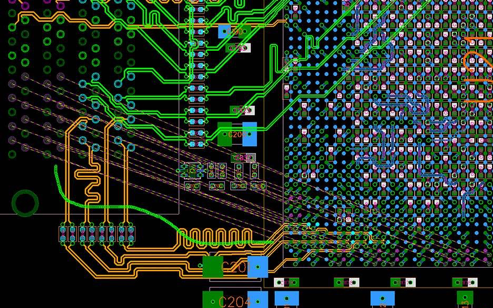
\includegraphics[width=6.5cm,height=5.5cm]{fig1}
	\caption{EDA is used in PCB board design for fast routing and global optimization}
	\label{Fig1}
\end{figure}
Compared with traditional digital circuit design methods, using EDA to design has many extraordinary characteristics and advantages. It adopts a top-down design method. The primary simulation and error correction processes of the design are completed at a high level, which is helpful for simple detection of structural design errors, thereby avoiding waste of time and cost in work. Also, the workload of logic function simulation is significantly reduced and design efficiency is lifted evidently. Hardware description language is an essential part of EDA technology and a utterly significant software tool in EDA design and development. One of the advantages of using it for electronic system design is that it allows designers to focus on the realization of their functions without spending too much time and effort on process-related factors. Figure 3 demonstrates the overall circuit layout of a certain project, making the advantage more distinct.
\begin{figure}[H]
	\centering
	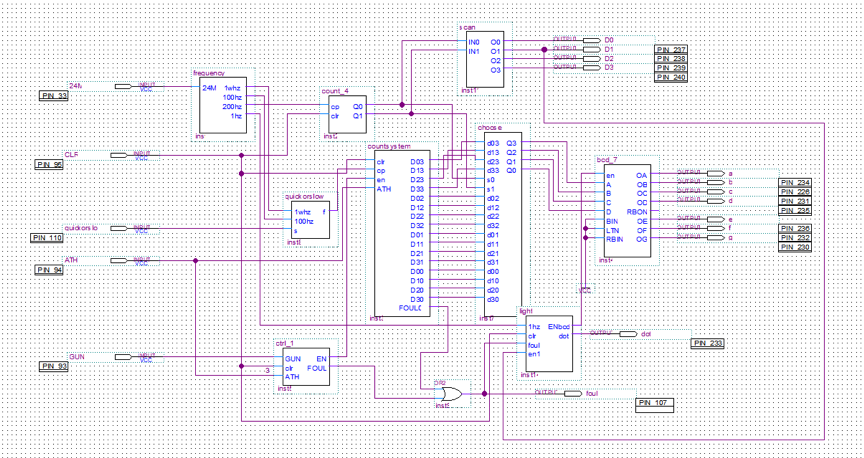
\includegraphics[width=8cm,height=6.5cm]{fig2}
	\caption{Circuit top-level block is designed in Quartus}
	\label{Fig2}
\end{figure}
% You must have at least 2 lines in the paragraph with the drop letter
% (should never be an issue)
Besides, its supporting hardware integration is high enough and the hardware has small sizes and consumes relatively low energy. It leads to not only low design costs, short design cycle, good design portability and high efficiency, but also convenience for teamwork.Regardless of the design process or the design results, it is worth trying to use the EDA mainstream development software Quartus to compile the program design. The experimental results also show that the solution is feasible. Furthermore, it is well implemented in the compilation environment of Quartus and the hardware condition of cyclone board. 

\section{Design Method}
% no \IEEEPARstart
% You must have at least 2 lines in the paragraph with the drop letter
% (should never be an issue)
\subsection{Verilog HDL}
Verilog generally refers to Verilog HDL. Verilog HDL is a Hardware Description Language (HDL), which describes the structure and behavior of digital system hardware in text form. It can be used to represent logical circuit diagrams, logical expressions, and the logical functions performed by digital logic systems.

Verilog was first designed to be a hardware description language with a basic syntax [3] similar to C. This is because C language has been widely used in many fields at the beginning of Verilog invention, and many language elements of C language have been well-received. Being similar to C makes it easier for circuit designers to learn and accept, although there are still many differences between Verilog and C. 

As a hardware description language different from ordinary computer programming languages, it has some unique language elements, such as vector nets and registers, non-blocking assignments in the process, and so on. In general, designers with a C language will be able to grasp the Verilog hardware description language quickly.

\subsection{Design Scheme Overview}
The design is to complete a calculator that can implement addition, subtraction, and multiplication between two signed two-digit decimal numbers. The input data range is from 0 to 99, and the range of calculation results is from -9081 to 9081. The realization of the calculator function is to input the first data by pressing the keys, select the corresponding calculation symbol, then enter the second data, and press the equal sign to get the corresponding result. 

It is found that most calculators in the current markets can only do a single-digit calculation, and they cannot process the addition and subtraction of negative numbers. This scheme is greatly improved and optimized on this basis. There is a total of five modules in this design plan, which respectively are input data module, calculation module, display module, transcoding module and control module. Based on the modular design idea, the top-down hierarchical design method is used for the project. The input signals include a key signal, a symbol signal, an equal signal, a zero signal and a negation signal. The output signal is the output data, which is the result of the calculation.
\begin{figure}[H]
	\centering
	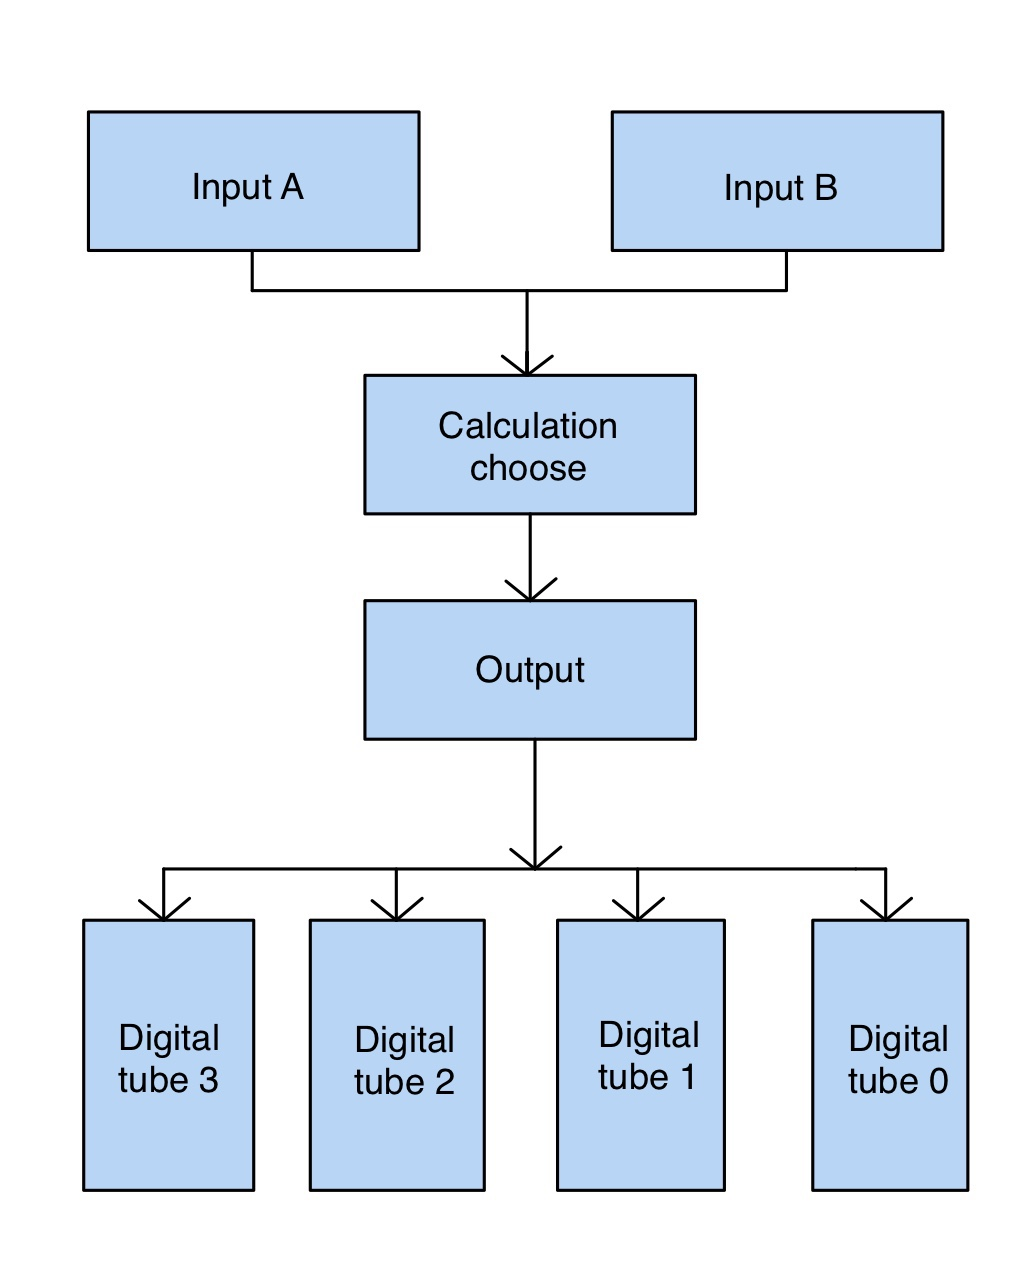
\includegraphics[width=6.5cm]{fig3}
	\caption{Mind mapping of the design explains how i achieve the purpose of the calculator}
	\label{Fig3}
\end{figure}
\subsubsection{Input Module Design}
\hfill\\
The one-digit calculator used a four-digit switch on the development board to indicate the number of the input data. For example, the levels of four switches, which are 1001, indicate that the data is 9. However, it is more difficult in reality to use them to show numbers because users do not have the time to convert what exactly the binary numbers of the input ones are, so i decided to increase the value of the input data by pressing keys. In order to avoid the trouble of converting two decimal numbers into two BCD codes, the design of the solution was to use two keys when inputting one data. One controlled the tens of the input data, and the other controlled the units. Each time the user clicks, the corresponding digit of the data is increased by one. What is more, it is more surprising that when the input data is relatively large, the number of key presses will be much less. Suppose that the input data is 78, instead of pressing the same key for 78 times, uses only need to press 15 times to adjust to the required number, saving pretty much time. 

When the complement signal is valid, the most significant digit of the seven-digit digital tube is only lit in the middle, which means that the number becomes negative and the g tube is red, as is shown in Figure 3. When the operator in need is selected and the calculation symbol signal is valid, only the least significant digit zero of the four-digit digital tube lights up, waiting for the second data to be input. The second data input process is the same as the first data operation. When the equal sign signal is valid, the calculation result can be output. If the set signal [4] is required during the process, the digital tube will display zero. 

\begin{figure}[H]
	\centering
	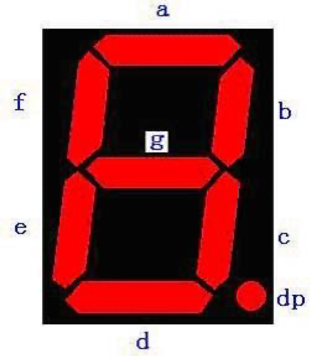
\includegraphics[width=5cm]{fig4}
	\caption{Structure of the digital tube is the reference for the codes}
	\label{Fig4}
\end{figure}
When compiling a language, two input data need to be represented by two variables. Because the design takes into account the problem of positive and negative signs, the sign bit is also included in the input data, and a signed variable is added. The data with the added sign bit is also a new variable, which needs to be defined in the module. 

In previous designs, many solutions chose to use keys as a carrier for inputting operator signals, and keys had to specify an intermediate variable to store the change in level. In programming languages, in order to reduce intermediate variables, switches were eventually selected as the input symbol to control the addition, subtraction, and multiplication symbols, making the program more concise and compiled faster and reducing the warnings accordingly.
\subsubsection{Calculation Module Design}
\hfill\\
There were not many factors to consider in the calculation module. For the corresponding symbols were already provided in the language, addition could be implemented directly in the programming language, and subtraction was to invert the original number and add one to the inverted number, which was quite simple. The code for multiplication was complicated and needed to be completed using related rules. At the beginning of the multiplication of two four-digit binary numbers, if the last bit of the second number is 0, the result is shifted directly to the left [5] by one bit. If the second bit of the data is 1, the current result is equal to the first data adding the current result and second data is moved one bit to the left. This process is repeated eight times and the result of the multiplication is obtained. The codes of the multiplication module are as follows:

always @ (M1, M2, CLR, R, P) 
	
	begin
	
	\qquad R = M2;
	
	\qquad P = 1'b0;
	
	\qquad if (CLR)
	
	\qquad P = 0;
	
	\qquad else begin
	
	\qquad \qquad \qquad repeat(8)
	
	\qquad \qquad  \qquad begin
	
	\qquad \qquad \qquad\qquad  P = P \textless \textless 1; 
	
	\qquad \qquad \qquad \qquad if(R[7])
	
	\qquad \qquad \qquad \qquad P = P + M1; 
	
	\qquad \qquad \qquad \qquad R = R \textless \textless 1;
	
	\qquad \qquad \qquad end
	
	\qquad \qquad end 
	
	end

\subsubsection{Transcoding Module Design}
\hfill\\
Because the sign bit calculation is added to this design, when the negation signal is valid, the module needs to negate and added one to the current binary data. When the data is input, units and tens are input separately. The BCD code is in need of being converted into a binary number to be calculated in the program. The final calculation result is binary, which requires to be converted into BCD code for display, and Figure 4 represents the process. In consideration of convenience, take the traditional one-digit decimal number calculator as an example, its results are divided into three types: negative one-digit numbers, positive one-digit ones, and positive two-digit ones.

When negative, the sign bit is 1, and the intermediate variable is used to invert the result, after which it is added one to get the units. When one-digit, the penultimate digit is 0, and the last digit shows that unit number. When two-digit, a method called shift and add three is time to use. If the calculator only needs to shift eight digits, so repeat 8. The codes judged whether every four digits are greater than 4, and if they are, three are added to get each bit, and units and tens are got. For a two-digit decimal number calculator, I repeated the above steps for 16 times.  
\begin{figure}[H]
	\centering
	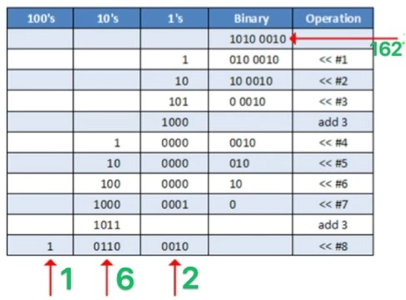
\includegraphics[width=9cm]{fig5}
	\caption{Schematic diagram of binary codes to BCD codes shows that the method is to shift the number and add three to it}
	\label{Fig5}
\end{figure}
If the final number is to be displayed on the FPGA development board, converting the BCD code into a seven-segment code is indispensable. This is the transcoding process that is necessary to be considered throughout the design.

\subsubsection{Display Module Design}
\hfill\\
The main problem of the display module is dynamic scanning. The program needed to scan the four digital tubes seen in Figure 5 continuously, which meant that they would be lit in turn. There was not only one bit at a time, but also the data result of that bit, which met the demand of dynamic scanning. During the scanning process, the binary number of the computer result was converted into BCD codes and then converted into seven-segment codes before it was displayed. This has been described in the transcoding module design above. When writing a program, a clock signal cannot be ignored. Every time the rising edge of the clock signal came, the bright digital tube of the four was replaced. Display modules are almost common parts of such FPGA programs, and the method is essentially the same thing.
\begin{figure}[H]
	\centering
	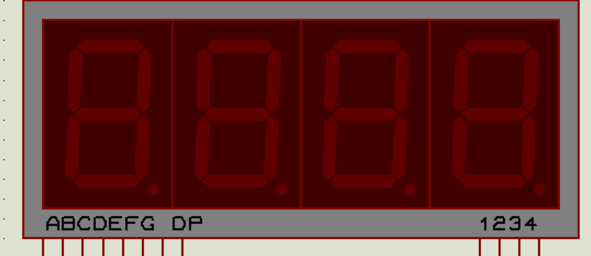
\includegraphics[width=8.5cm]{fig6}
	\caption{Display of four-digit digital tubes}
	\label{Fig6}
\end{figure}

\subsubsection{Control Module Design}
\hfill\\
In the control module, the program Design of controls whether the first number or the second number was input when the key was pressed. It means that the operator is required to enter. Otherwise, it is the first data. It also controls whether addition, subtraction, or multiplication is performed. If one of the addition and subtraction signals is valid, the control program performs that operation. At the same time, whether the data is cleared or not is commanded by the controller. Before entering the first data and before entering the second data, the nixie tube should show zero and only in the least significant position. Controlling the display of excessive zeros is also an important function of the control module, that is, determining whether the high level is zero. If it is, the digital tube was dimmed. If it is not, it continues to determine the next high-level data, which is more in line with the user habits. It can display four digits when calculating, but when the calculation result is less than four digits, the previous digits are prevented from being displayed. For such improvements, adding some 'always' drivers in the program was enough.

\subsubsection{Experimental Optimization Design}
\hfill\\
Real problems were founded after downloading the program to the FPGA development board for experiments. Due to the hardware limitations of the development board, the buttons and switches had the corresponding jitter. This was especially obvious when entering data. When a key was pressed, the data increased by more than 1, but a random number, because the key jumped slightly up and down during the pressing process, which caused the key signal to be valid for a couple of times. Although the switch also had a problem of instability, since not involved in the display field, it was not necessary to take optimization measures. 

The switch used for the normal button was a mechanical elastic switch. When the mechanical contact is opened or closed, due to the elastic effect of the mechanical contact, a key switch will not turn on steadily immediately [6] when it is closed. Therefore, there was a series of jitters at the moment of closing and opening. The measure to prevent this phenomenon was to depress the keys.
\begin{figure}[H]
	\centering
	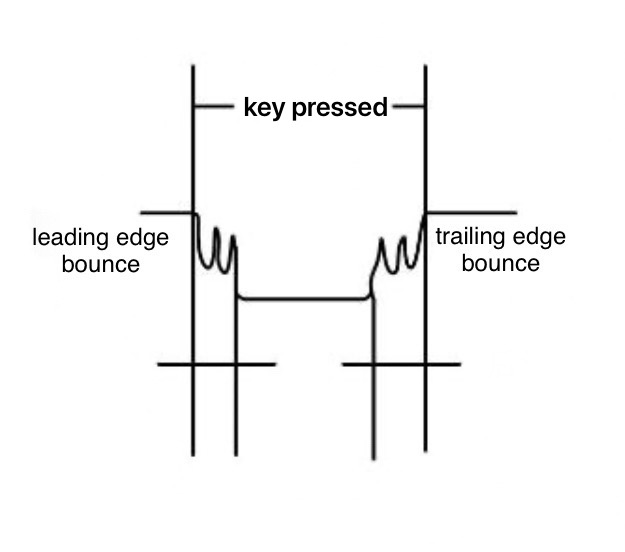
\includegraphics[width=7.5cm]{fig7}
	\caption{Schematic of button jitter}
	\label{Fig7}
\end{figure}
Because software debounce is more convenient and does not require additional hardware overhead, it is generally used. The software debounce method commonly used in single-chip microcomputers was actually very simple. After the single-chip microcomputer obtains the information that the port is low, it is not immediately determined that the button is pressed, but it is tested again after a delay of 10ms or longer. If the port is still low, it means that the key was indeed pressed. This avoids the jitter time when the key is pressed, and when the port is detected to be high after the key is released, it is delayed for another 50ms. Eliminate the jitter on the back edge, and then process the keys. Nevertheless, in general, the back edge of the key release is usually not processed. The practice has proved that it can meet the daily requirements.

\begin{figure}[H]
	\centering
	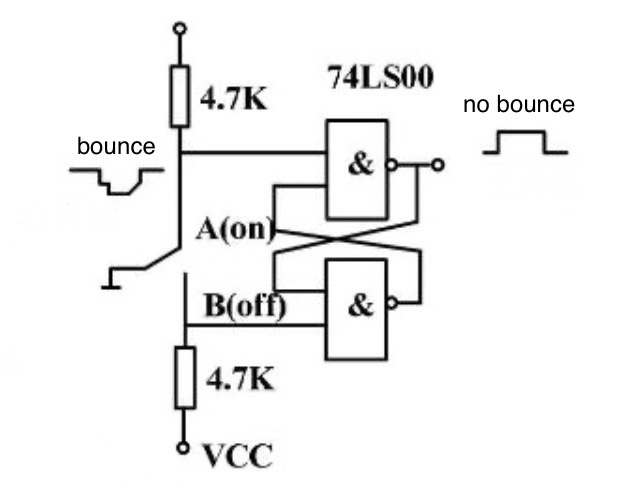
\includegraphics[width=7.5cm]{fig8}
	\caption{Hardware debounce circuit}
	\label{Fig5}
\end{figure}

In the input module, the measure taken in this solution was the de-jittering program, which introduced an intermediate variable called count. This signal will increase by one as long as the button is shaken. It was only effective when the button was pressed, and the variable was equal to a certain number, after which the count variable changed to zero. This improved the situation of button shake to a certain extent.

\section{Results}
\subsection{Operating Steps}
The results of the design were shown in the steps.

Step1: Download the file obtained after the pins are assigned to the FPGA board. After the download is successful, one zero is displayed on the board. Increase the single-digit value by controlling the ones button at this time. To change the ten digits, press the ten-digit button, and input the first data 46.

Step2: Choose to dial the next operation symbol. For example, dial the plus switch.

Step3: Then enter the second data the same way as the first data. Suppose that the data is 67, and then press a sign button, it becomes -67. The negative sign is displayed at the highest position.

Step4: Press the equal switch to show the sign to get the final result -21. The negative sign is in the highest position, 21 is respectively at the penultimate position and the penultimate position.

Step5: Press the clear signal to reset, the display result is 0, in the lowest position. A new round of calculations can be performed.
\subsection{Demonstration}
The experimental results perfectly met the expectations, and the correct calculation results were obtained. 
\subsection{Defect}
The problem of key jitter was better overcome when inputting data and inputting operator signals.But this calculator cannot proceed continuous addition, subtraction, and multiplication. However, since the calculator does not have similar functions in real life and does not need to use similar functions, it was not designed accordingly in this experiment.

\section{Conclusion}
This experiment can implement addition, subtraction, and multiplication between two signed two-digit decimal numbers. Taking into account the actual reading habits, the high zero suppression is not displayed during the design display process. The design process is slightly complicated, but the design goals are well accomplished. And most of the calculators on the market have been improved and functions have been expanded. In the design of the experiment, it should be noted that a highly important idea in the hardware description is the design of the modules. Sub-modules make the code clearer and more convenient to call, improve the efficiency of the code and the ability to correct errors, and save the time of designers. The rapid development of EDA tools has brought great convenience to the design of digital circuits.
% use section* for acknowledgment
\ifCLASSOPTIONcompsoc
% The Computer Society usually uses the plural form
\section*{Acknowledgments}
% regular IEEE prefers the singular form
We acknowledge the effort from the authors of the Verilog Learning. These resources make this project in the wild possible. This design was supported by the Programmable Tools Center of Fudan University.




% An example of a floating figure using the graphicx package.
% Note that \label must occur AFTER (or within) \caption.
% For figures, \caption should occur after the \includegraphics.
% Note that IEEEtran v1.7 and later has special internal code that
% is designed to preserve the operation of \label within \caption
% even when the captionsoff option is in effect. However, because
% of issues like this, it may be the safest practice to put all your
% \label just after \caption rather than within \caption{}.
%
% Reminder: the "draftcls" or "draftclsnofoot", not "draft", class
% option should be used if it is desired that the figures are to be
% displayed while in draft mode.
%
%\begin{figure}[!t]
%\centering
%\includegraphics[width=2.5in]{myfigure}
% where an .eps filename suffix will be assumed under latex, 
% and a .pdf suffix will be assumed for pdflatex; or what has been declared
% via \DeclareGraphicsExtensions.
%\caption{Simulation results for the network.}
%\label{fig_sim}
%\end{figure}

% Note that the IEEE typically puts floats only at the top, even when this
% results in a large percentage of a column being occupied by floats.


% An example of a double column floating figure using two subfigures.
% (The subfig.sty package must be loaded for this to work.)
% The subfigure \label commands are set within each subfloat command,
% and the \label for the overall figure must come after \caption.
% \hfil is used as a separator to get equal spacing.
% Watch out that the combined width of all the subfigures on a 
% line do not exceed the text width or a line break will occur.
%
%\begin{figure*}[!t]
%\centering
%\subfloat[Case I]{\includegraphics[width=2.5in]{box}%
%\label{fig_first_case}}
%\hfil
%\subfloat[Case II]{\includegraphics[width=2.5in]{box}%
%\label{fig_second_case}}
%\caption{Simulation results for the network.}
%\label{fig_sim}
%\end{figure*}
%
% Note that often IEEE papers with subfigures do not employ subfigure
% captions (using the optional argument to \subfloat[]), but instead will
% reference/describe all of them (a), (b), etc., within the main caption.
% Be aware that for subfig.sty to generate the (a), (b), etc., subfigure
% labels, the optional argument to \subfloat must be present. If a
% subcaption is not desired, just leave its contents blank,
% e.g., \subfloat[].


% An example of a floating table. Note that, for IEEE style tables, the
% \caption command should come BEFORE the table and, given that table
% captions serve much like titles, are usually capitalized except for words
% such as a, an, and, as, at, but, by, for, in, nor, of, on, or, the, to
% and up, which are usually not capitalized unless they are the first or
% last word of the caption. Table text will default to \footnotesize as
% the IEEE normally uses this smaller font for tables.
% The \label must come after \caption as always.
%
%\begin{table}[!t]
%% increase table row spacing, adjust to taste
%\renewcommand{\arraystretch}{1.3}
% if using array.sty, it might be a good idea to tweak the value of
% \extrarowheight as needed to properly center the text within the cells
%\caption{An Example of a Table}
%\label{table_example}
%\centering
%% Some packages, such as MDW tools, offer better commands for making tables
%% than the plain LaTeX2e tabular which is used here.
%\begin{tabular}{|c||c|}
%\hline
%One & Two\\
%\hline
%Three & Four\\
%\hline
%\end{tabular}
%\end{table}


% Note that the IEEE does not put floats in the very first column
% - or typically anywhere on the first page for that matter. Also,
% in-text middle ("here") positioning is typically not used, but it
% is allowed and encouraged for Computer Society conferences (but
% not Computer Society journals). Most IEEE journals/conferences use
% top floats exclusively. 
% Note that, LaTeX2e, unlike IEEE journals/conferences, places
% footnotes above bottom floats. This can be corrected via the
% \fnbelowfloat command of the stfloats package.








% conference papers do not normally have an appendix







% trigger a \newpage just before the given reference
% number - used to balance the columns on the last page
% adjust value as needed - may need to be readjusted if
% the document is modified later
%\IEEEtriggeratref{8}
% The "triggered" command can be changed if desired:
%\IEEEtriggercmd{\enlargethispage{-5in}}

% references section

% can use a bibliography generated by BibTeX as a .bbl file
% BibTeX documentation can be easily obtained at:
% http://mirror.ctan.org/biblio/bibtex/contrib/doc/
% The IEEEtran BibTeX style support page is at:
% http://www.michaelshell.org/tex/ieeetran/bibtex/
%\bibliographystyle{IEEEtran}
% argument is your BibTeX string definitions and bibliography database(s)
%\bibliography{IEEEabrv,../bib/paper}
%
% <OR> manually copy in the resultant .bbl file
% set second argument of \begin to the number of references
% (used to reserve space for the reference number labels box)
\begin{thebibliography}{1}
\bibitem{IEEEhowto:kopka}
Zhou, X. \& Hao, X. \& Liu, S. \& Wang, J. \& Xu, J. \& Hu, J. (2014). Design of Washing Machine Controller Based on VHDL. 194.10.1117/12.2780289. 
\bibitem{IEEEhowto:kopka}
Alex, H. \& Ilya, B. \& Hg, F.. (2015). Digital Circuit Design Guide. Proceedings of EDA, IEEE, EDA System Foundation. 1097-1105. 
\bibitem{IEEEhowto:kopka}
Howard, A. G., Zhu, M., Chen, B., Kalenichenko, D., Wang, W., Weyand, T., Andreetto, M. \& Adam, H. (2019). MobileNets: Efficient Compiling Languages for FPGA, arXiv:1704.04861 [cs.CV].
\bibitem{IEEEhowto:kopka}
Wang, L., Xiong, Y. \& Wang, Z., Qiao, Y. \& Lin, D., Tang, X. \& Gool, L. V. (2016). Temporal Segment Networks: Towards Good Practices for FPGA designs. Computer Tools – ECCV 2016 Lecture Notes in Computer Science, 19–32. doi: 10.1087/978-3-319-46484-8\_2.
\bibitem{IEEEhowto:kopka}
Feichtenhofer, C. \& Pinz, A. \& Zisserman, A. (2016). Experiments on FPGA Board, 2016 IEEE Conference on EDA tools (CVPR).



\end{thebibliography}




% that's all folks
\end{document}


